\begin{figure}[H]
\centering
\includegraphics[page=8,width=0.4\textwidth]{\FCNCFigures/tthML/showFake/faketau/postfit/NOMINAL/reg1l1tau1b2j_os_vetobtagwp70_highmet/chi2.pdf}
\put(-100, 80){\textbf{(a)}}
\put(-90, 95){\footnotesize{$t_h\tlhad$-2j}}
\includegraphics[page=8,width=0.4\textwidth]{\FCNCFigures/tthML/showFake/faketau/postfit/NOMINAL/reg1l1tau1b3j_os_vetobtagwp70_highmet/chi2.pdf}
\put(-100, 80){\textbf{(b)}}
\put(-90, 95){\footnotesize{$t_h\tlhad$-3j}}\\
\includegraphics[page=6,width=0.4\textwidth]{\FCNCFigures/xTFW/showFake/NOMINAL/reg2mtau1b2jos_vetobtagwp70_highmet/chi2.pdf}
\put(-100, 80){\textbf{(c)}}
\put(-90, 95){\footnotesize{$t_h\thadhad$-2j}}
\includegraphics[page=6,width=0.4\textwidth]{\FCNCFigures/xTFW/showFake/NOMINAL/reg2mtau1b3jos_vetobtagwp70_highmet/chi2.pdf}
\put(-100, 80){\textbf{(d)}}
\put(-90, 95){\footnotesize{$t_h\thadhad$-3j}}
\caption{ Comparison of the distributions of $\chi^2$ in Eq. \ref{eq:eq2} in the  leptonic channel (a,b) and  hadronic channel (c,d). The real tau contributions shown from ttbar and other MC including diboson, single top, and V+jets. Only
statistical uncertainties are being shown. Underflow and overflow bins are included respectively in the first and last bins.}
\label{fig:chi2}
\end{figure}
